\begin{figure}[h]
  \centering

  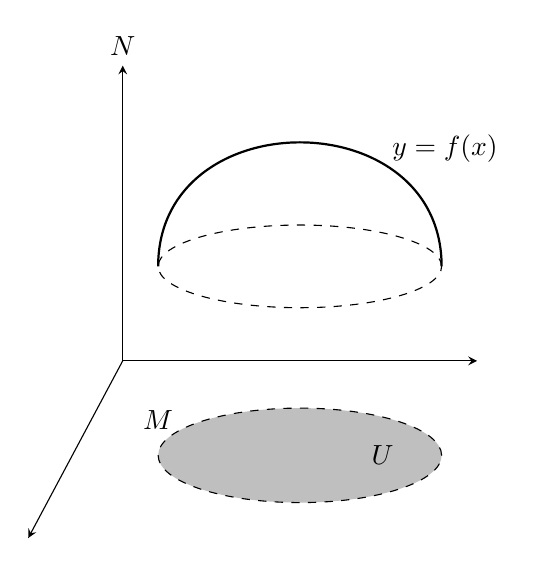
\begin{tikzpicture}[scale=1.5, >=stealth]

    % --- The Axes (simulating 3D with 2D lines) ---
    % Vertical Axis
    \draw[->] (0,0) -- (0,2.5) node[above] {$N$};
    % Horizontal-ish Axis
    \draw[->] (0,0) -- (3,0);
    % Tilted "depth" Axis
    \draw[->] (0,0) -- (-0.8,-1.5);

    % --- Manifold M area ---
    % Domain U: a 2D ellipse tilted to look like it's on a plane
    \filldraw[fill=gray!50, draw=black, dashed] (1.5, -0.8) ellipse (1.2 and 0.4);
    \node at (2.2, -0.8) {$U$};
    \node at (0.3, -0.5) {\textbf{$M$}};

    % --- The Graph y = f(x) ---
    % The base of the "dome" (dashed ellipse)
    \draw[dashed] (1.5, 0.8) ellipse (1.2 and 0.35);

    % The upper curve (the graph line)
    % Using a simple arc or plot to represent the dome
    \draw[thick] (0.3, 0.8) .. controls (0.3, 2.2) and (2.7, 2.2) .. (2.7, 0.8);

    % Label for the graph
    \node[right] at (2.2, 1.8) {$y = f(x)$};

  \end{tikzpicture}

  \caption{An embedded submanifold}
  \label{fig:embedded_submanifold}
\end{figure}
